\clearpage
\section{Memory Address Translation}\label{page:memory-address-translation}\label{section:memory-address-translation}

Memory address translation is a separate pipeline after effective-address calculation. Effective-address evaluation
produces an address value or operand designator; segmentation optionally turns that value into a (:term:base.terms.linear_address:), and
paging optionally turns the (:term:base.terms.linear_address:) into a (:term:base.terms.memory_system_address:).

Instruction fetches use CS, stack accesses use SS, and (:term:base.terms.ordinary:) data accesses use the operation default data segment
unless an effective-address form explicitly selects another segment. SP and PC forms use their fixed segments.

(:ref:base.instructions.SEGLEA:) exposes the (:term:base.terms.linear_address:) produced by (:term:base.terms.segment_pre_translation:) when
software explicitly needs it. Its instruction description defines the point check, FLAGS result, destination
suppression, and auto-update commit behavior. SEGLEA applies (:term:base.terms.segment_pre_translation:) to the computed starting point.

\begin{center}\vspace{3pt}
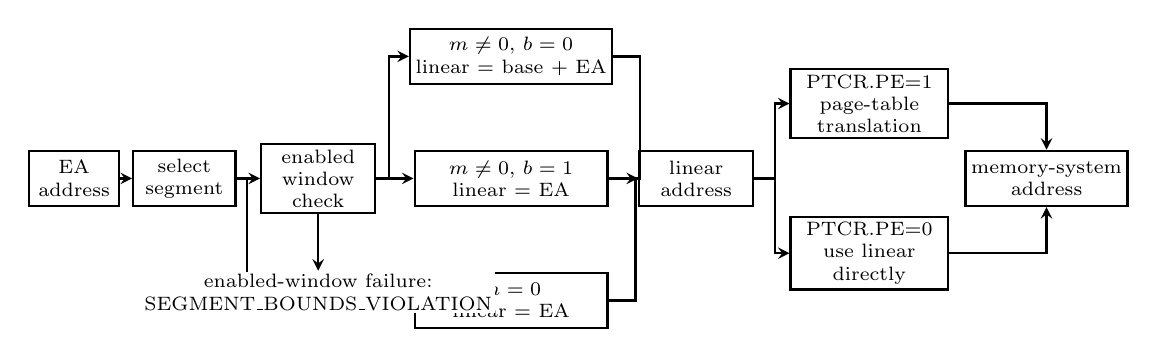
\begin{tikzpicture}[x=1cm,y=1cm,every node/.style={font=\scriptsize},>=stealth,line width=0.82pt]
\tikzset{box/.style={draw,align=center,minimum height=0.70cm,inner sep=2pt}, lab/.style={fill=white,inner sep=1pt}}
\node[box,minimum width=1.15cm] (ea) at (0.55,0) {EA\\address};
\node[box,minimum width=1.30cm] (sel) at (1.95,0) {select\\segment};
\node[box,minimum width=1.45cm] (check) at (3.65,0) {enabled\\window\\check};
\node[box,minimum width=2.45cm] (add) at (6.10,1.55) {$m\ne0$, $b=0$\\linear = base + EA};
\node[box,minimum width=2.45cm] (keep) at (6.10,0) {$m\ne0$, $b=1$\\linear = EA};
\node[box,minimum width=2.45cm] (disabled) at (6.10,-1.55) {$m=0$\\linear = EA};
\node[box,minimum width=1.45cm] (lin) at (8.45,0) {linear\\address};
\node[box,minimum width=2.00cm] (page) at (10.65,0.95) {PTCR.PE=1\\page-table\\translation};
\node[box,minimum width=2.00cm] (direct) at (10.65,-0.95) {PTCR.PE=0\\use linear\\directly};
\node[box,minimum width=1.75cm] (out) at (12.90,0) {memory-system\\address};
\draw[->] (ea.east) -- (sel.west);
\coordinate (modebranch) at (2.75,0);
\draw (sel.east) -- (modebranch);
\draw[->] (modebranch) -- (check.west);
\draw[->] (modebranch) |- node[lab,pos=0.82,above] {$m=0$: disabled} (disabled.west);
\coordinate (segbranch) at (4.55,0);
\draw[->] (check.east) -- (segbranch) |- (add.west);
\draw[->] (check.east) -- (keep.west);
\draw[->] (check.south) -- ++(0,-0.72) node[lab,below,align=center] {enabled-window failure:\\SEGMENT\_BOUNDS\_VIOLATION};
\coordinate (linmerge) at (7.45,0);
\draw (add.east) -- ++(0.34,0) |- (linmerge);
\draw (keep.east) -- (linmerge);
\draw (disabled.east) -- ++(0.34,0) |- (linmerge);
\draw[->] (linmerge) -- (lin.west);
\coordinate (pebranch) at (9.45,0);
\draw[->] (lin.east) -- (pebranch) |- (page.west);
\draw[->] (lin.east) -- (pebranch) |- (direct.west);
\draw[->] (page.east) -| (out.north);
\draw[->] (direct.east) -| (out.south);
\end{tikzpicture}
\BedrockFigureCaption{Address Translation Pipeline}
\end{center}

